\documentclass[9pt,twocolumn,twoside,lineno]{pnas-new}
% Use the lineno option to display guide line numbers if required.
% Note that the use of elements such as single-column equations
% may affect the guide line number alignment. 

%Many authors find it useful to organize their manuscripts with the following order of sections;  Title, Author Affiliation, Keywords, Abstract, Significance Statement, Results, Discussion, Materials and methods, Acknowledgments, and References. Other orders and headings are permitted.

\usepackage[super]{nth} %adds superscripts for things like 20th

\templatetype{pnasresearcharticle} % Choose template 
% {pnasresearcharticle} = Template for a two-column research article
% {pnasmathematics} = Template for a one-column mathematics article
% {pnasinvited} = Template for a PNAS invited submission

\title{The Changing Character of Banded Rainfall in Eastern China, 1951-2007}

% Use letters for affiliations, numbers to show equal authorship (if applicable) and to indicate the corresponding author
\author[a,1]{Jesse Day}
\author[a]{Inez Fung} 
\author[b]{Weihan Liu}

\affil[a]{Department of Earth and Planetary Science, University of California Berkeley, 94103}
\affil[b]{College of Letters and Sciences, University of California Berkeley, 94103}

%\subsection*{Author Affiliations}

%Include department, institution, and complete address, with the ZIP/postal code, for each author. Use lower case letters to match authors with institutions, as shown in the example. Authors with an ORCID ID may supply this information at submission.

% Please give the surname of the lead author for the running footer
\leadauthor{Day} 

% Please add here a significance statement to explain the relevance of your work
\significancestatement{Eastern China experienced a late-twentieth-century change in rainfall known as the ``South Flood-North Drought.'' We employ a novel image processing algorithm that detects rainbands, a key component of summer Chinese weather, and also classifies rainfall as either banded or local. Changes in the frequency of banded rainfall contributed most to rainfall changes across 1951-2007, with an uptick in banded rainfall intensity after 1993. In contrast, there is no significant trend in local rainfall. We hope to provide a new framework for diagnosis of the relative impacts of global warming, aerosols and natural variability by supplying an improved portrait of historical rainfall change.}

% Please include corresponding author, author contribution and author declaration information
\authorcontributions{J.D. developed the algorithm and produced data; J.D. and I.F. contributed equally to the interpretation of results; W.L. contributed to algorithm development; }
\authordeclaration{The authors declare no conflict of interest.}
\correspondingauthor{\textsuperscript{2}To whom correspondence should be addressed. E-mail: jessed@berkeley.edu}

% Keywords are not mandatory, but authors are strongly encouraged to provide them. If provided, please include two to five keywords, separated by the pipe symbol, e.g:
\keywords{East Asian Monsoon|Monsoons|Rainfall|Rainbands|New Methods} 

\begin{abstract}
The topography and continental configuration of East Asia favor the year-round existence of zonal storm tracks that extend thousands of miles from China into the northwestern Pacific Ocean. In spring and summer, when they are referred to as the ``Meiyu Front,'' these rainbands intensify and shift northward through a series of rainfall stages collectively known as the East Asian summer monsoon. Using a new technique called the Rainband Detection Algorithm (RDA), we create a daily catalog of all rainband occurrences in East China during 1951-2007 (20,819 days total), quantify their attributes, and classify all rainfall on each day as either ``banded'' or ``local'' rainfall. Our climatology shows that the East Asian summer monsoon consists of a series of coupled changes in rainband frequency, latitude and intensity. Furthermore, significant decadal rainfall changes in East China are overwhelmingly due to changes in banded rainfall. These changes in banded rainfall can further be decomposed into changes in frequency and intensity. We attribute the ``South Flood-North Drought'' pattern observed beginning in the 1980s to changes in the frequency of rainbands, while the years 1994-2007 witnessed an uptick in rainband intensity relative to the rest of the study years. Meanwhile, trends in local rainfall are found to be insignificant. We suggest that this particular signature of rainfall changes could reflect a particular large-scale forcing such as global warming or aerosol loading.
\end{abstract}

\dates{This manuscript was compiled on \today}
\doi{\url{www.pnas.org/cgi/doi/10.1073/pnas.XXXXXXXXXX}}

\begin{document}

% Optional adjustment to line up main text (after abstract) of first page with line numbers, when using both lineno and twocolumn options.
% You should only change this length when you've finalised the article contents.
\verticaladjustment{-2pt}

\maketitle
\thispagestyle{firststyle}
\ifthenelse{\boolean{shortarticle}}{\ifthenelse{\boolean{singlecolumn}}{\abscontentformatted}{\abscontent}}{}

\dropcap{E}astern China receives about 60\% of its precipitation from May to August via the East Asian summer monsoon. The period of peak rainfall lasting from early June to mid-July is called ``Meiyu season'' (lit. ``plum rains,'' referring to the spectacular growth of plum blossoms in central China with the onset of heavy rains). During this time, heavy rainfall occurs in zonal bands resulting from frontal synoptic conditions (the ``Meiyu Front''). The rainfall climatology of Japan and Korea also features similar meteorological phenomena known as the Baiu and Changma respectively. The contribution from these rainbands leads to a rainfall seasonality in the East Asian monsoon that is unique relative to other monsoon circulations \citep{Ding2005}. More generally, rainbands are a year-round feature of East Asian rainfall, attributed to the interplay between the East Asian tropospheric jet and Tibetan Plateau \citep{Molnar2010,Sampe2010,Chen2014}.
	 	  	 
	We have developed an image processing algorithm, the Rainband Detection Algorithm (RDA), which locates rainbands in daily precipitation maps and quantifies attributes such as latitude and intensity. By applying this algorithm to 57 years of daily weather station data for East China (defined as 105$^{\circ}$E-123$^{\circ}$E and 20$^{\circ}$N-40$^{\circ}$N), we create a database all of rainband occurrences in China and obtain a climatology of latitude, intensity.  All rainfall on each day is further classified as ``banded'' or ''local'' based on proximity to a detected rainband. We present for the first time a climatology of rainbands and banded rainfall (Figure~\ref{fig:hov_climo}). We also investigate several decadal changes, in particular the ``South Flood-North Drought'' phenomenon reported in East China post-1980 \citep{Hu1997,Gong2002,Nigam2013}, and also another reported change in behavior between 1994-2007 and 1980-1993 \citep{Kajikawa2012,Zou2015}. Several previous studies have compiled information on the variability of the Meiyu front on decadal and centennial timescales \citep{Chen2004,Ge2008,Xu2009}, but to our knowledge no previous author has compiled a multi-decadal catalog of rainband events.

%%FIGURE 1 Hovm�ller diagram of Meiyu latitude occupancy, 1951-2007. Produced by MATLAB scripts meiyufig1.m and meiyustats_compact.m.
\begin{figure}[htbp]
\centering
\noindent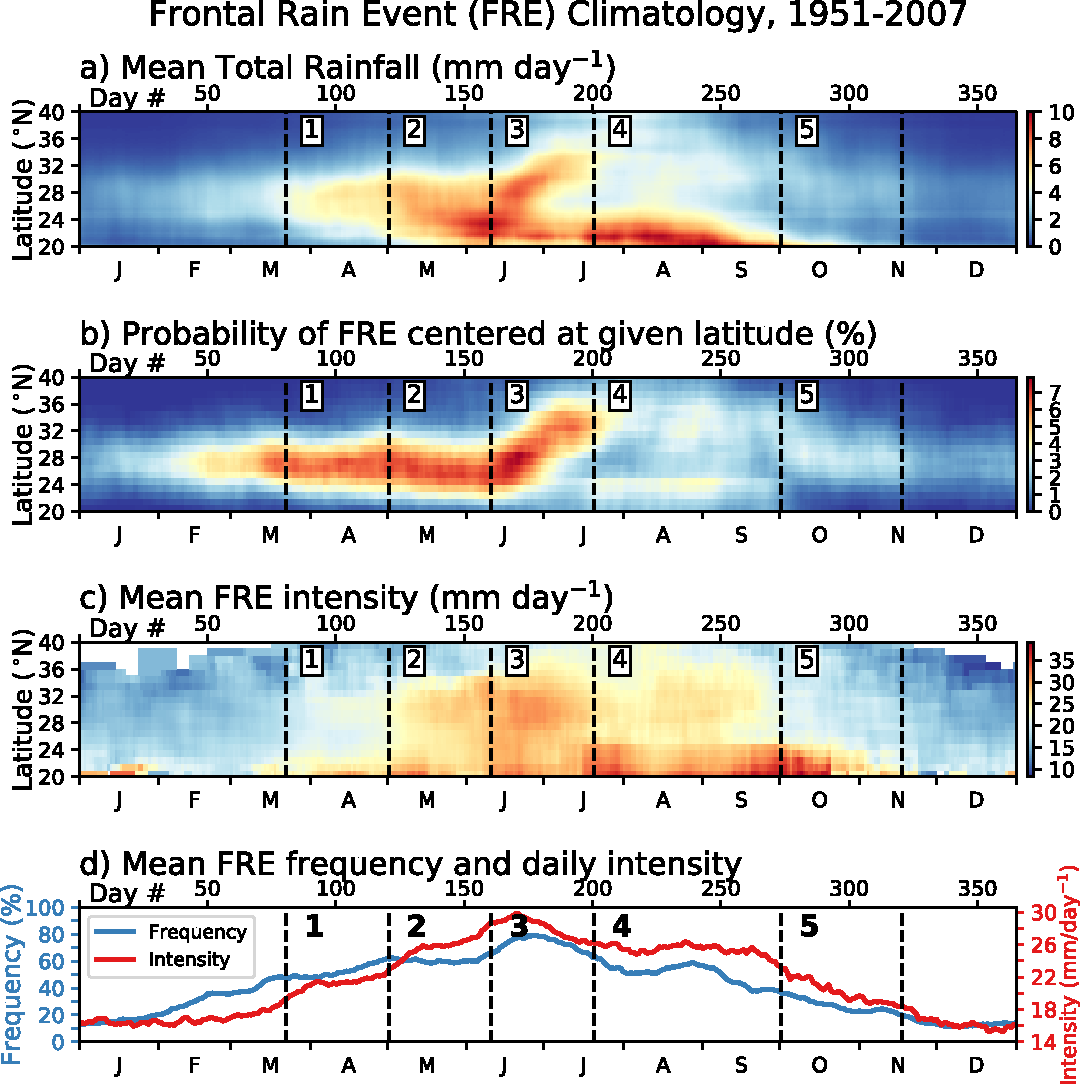
\includegraphics[width=\linewidth]{Figures/PNAS_climo_cropped}
\caption{Climatology of East Asian rainfall and rainbands, 1951-2007, with important time periods marked as follows: 1 - Spring Rains; 2 - Pre-Meiyu; 3 - Meiyu; 4 - Post-Meiyu; 5 - Fall Rains. a) Hovm\"oller diagram of precipitation (100-123$^{\circ}$E longitudinal average); b) Hovm\"oller diagram of probability of observing a rainband at a given latitude, smoothed in time with a 9-day and 2$^{\circ}$-running box filter; c) Mean rainband intensity (average of intensity of all rainbands within 15 days and +/-2.5$^{\circ}$ of latitude); d) Rainband frequency (15-day running mean) and mean intensity on each day.}
\label{fig:hov_climo}
\end{figure}

\section*{Rainband Climatology}

	We compile our daily rainband catalog into a 57-year daily climatology (1951-2007). The yearly progression of precipitation over eastern China is shown in Figure~\ref{fig:hov_climo}a and can be compared with reference \cite{Ding2005}. Abrupt climatological shifts in rainfall and rainband climatology frequently co-occur. Rainbands appear in all months, with maximum frequency and intensity in late June (80\%, mean of 31 mm day$^{-1}$) and a minimum in January (10\% and mean intensity of 12 mm day$^{-1}$). We define 5 periods of distinct behavior as demarcated in Figure~\ref{fig:hov_climo}, with the Pre-Meiyu, Meiyu and Post-Meiyu equivalent to the three stages of Meiyu rainfall described in reference \cite{Ding2005}:

\begin{enumerate}

\item The Spring Rains (days 60-120, March 1-April 30), previously studied in reference \cite{Tian1998}, marked by frequent but relatively weak rainbands (47\% occurrence, 20 mm day$^{-1}$ mean);

\item Pre-Meiyu season (days 121-160, May 1-June 9), during which rainfall and front intensity steadily increase (56\% occurrence, 25.5 mm day$^{-1}$ mean);

\item Meiyu season (days 161-200, June 10-July 19) when a remarkable 7-degree northward shift in mean rainband latitude occurs over the course of several weeks, and rainband frequency and intensity peaks (66\% occurrence, 28.3 mm day$^{-1}$ mean); 

\item Post-Meiyu season (days 201-273, July 20-September 30), when rainbands are less common than during the Spring Rains (42\% occurrence) but double rainbands occur more frequently (28\% chance of observing a secondary rainband if a primary rainband is observed); 

\item The Fall Rains (days 274-320, October 1-November 16), when mean rainband latitude shifts back southward from its northern maximum of 30$^\circ$N and rainband frequency decreases to just 27\%. 

\end{enumerate}

	These time periods are chosen subjectively, but our subsequent analysis is not dependent on their exact duration. Unlike other monsoonal regions, which tend to be very dry in winter \citep{Wang2002}, Eastern China receives about 40\% of yearly precipitation between September and April. Our estimate of onset day of Meiyu season roughly matches that estimated in \cite{Xu2009}. The Pre-Meiyu to Meiyu and Meiyu to Post-Meiyu transitions both entail rapid northward migrations in preferred location of banded rainfall (Figure~\ref{fig:type_climo}b). During days 160-180, likelihood of observing a rainfall maximizes between 26$^\circ$ and 30$^\circ$N, yet by days 200-220, the same region is less likely than any other latitude to feature a rainband (an 80\% decline in rainband frequency, and a decline in total rainfall from 7.6 mm day$^{-1}$ to 4.1 mm day$^{-1}$).

%%FIGURE 2 Decadal mean in different rainfall types during different time periods
\begin{figure}[htb]
\centering
\noindent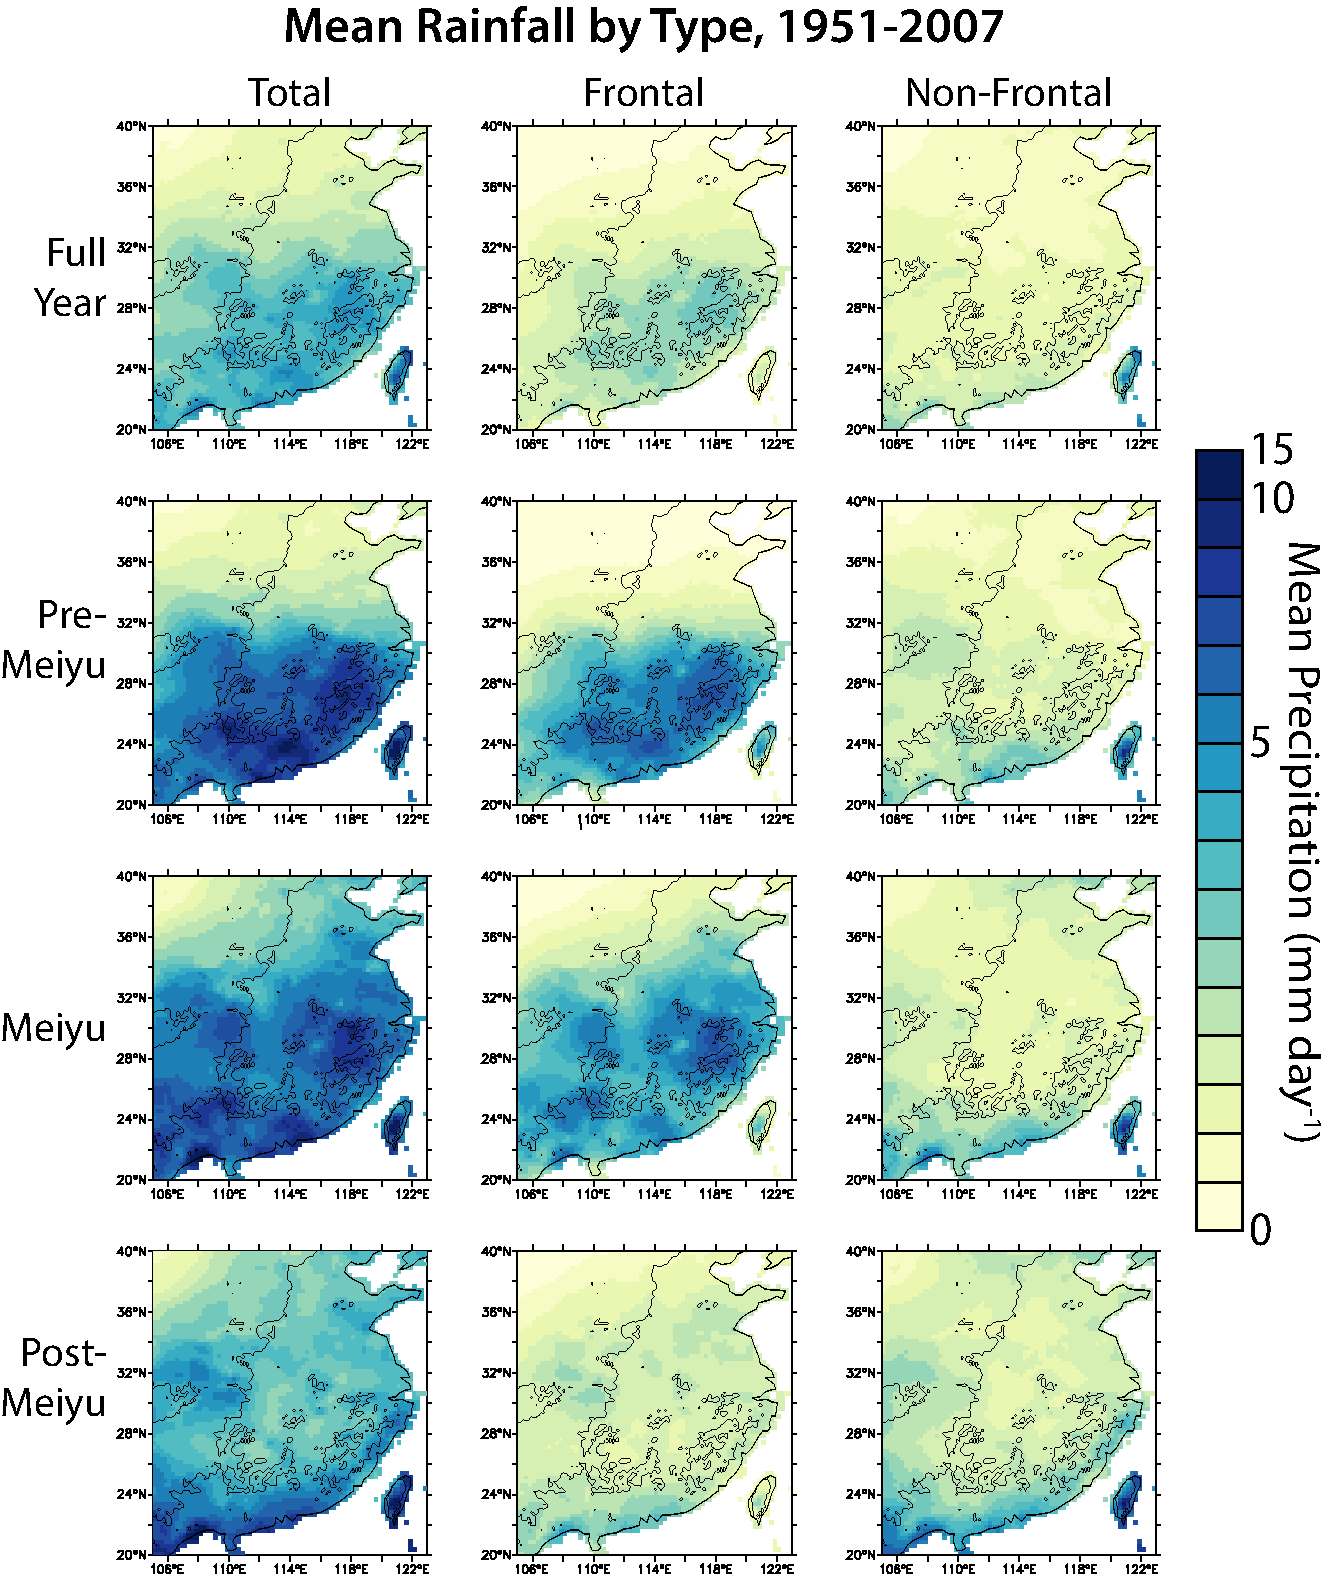
\includegraphics[width=\linewidth]{Figures/type_climo}
\caption{Climatology of the amount of total rainfall, banded rainfall and local rainfall for the full year, Pre-Meiyu (days 121-160), Meiyu (days 161-200) and Post-Meiyu (days 201-273). \textit{Banded} rainfall consists of all rainfall falling within 4$^{\circ}$ of a rainband axis and rainfall at any other adjacent point exceeding 10 mm day$^{-1}$. \textit{Local} rainfall includes all rainfall not meeting these criteria. Note that color bar switches from .5 to 1 mm day$^{-1}$ increment past 5 mm day$^{-1}$.}
\label{fig:type_climo}
\end{figure}
	
	Rainbands are generally more probable and stronger during spring than in fall, with notable intensity jumps around days 120 and 160. Some periods of heavy rainfall, in particular the August peak over southeastern China (>10 mm day$^{-1}$ around 20$^{\circ}$N), do not correspond to a surge in rainband frequency. Instead, August and September are known as the months when northwestern Pacific typhoons reach mainland China, which tend to leave locally favorable rainfall conditions in their wake \citep{Chen2007,Chen2011}. The most intense rainband events occur at low latitudes during October (days 270-300) during peak cyclone season \citep{Liu2003}.
	
%%FIGURE 3 Decadal changes in different rainfall types
\verb|
\begin{figure*}[tp]
\centering
\noindent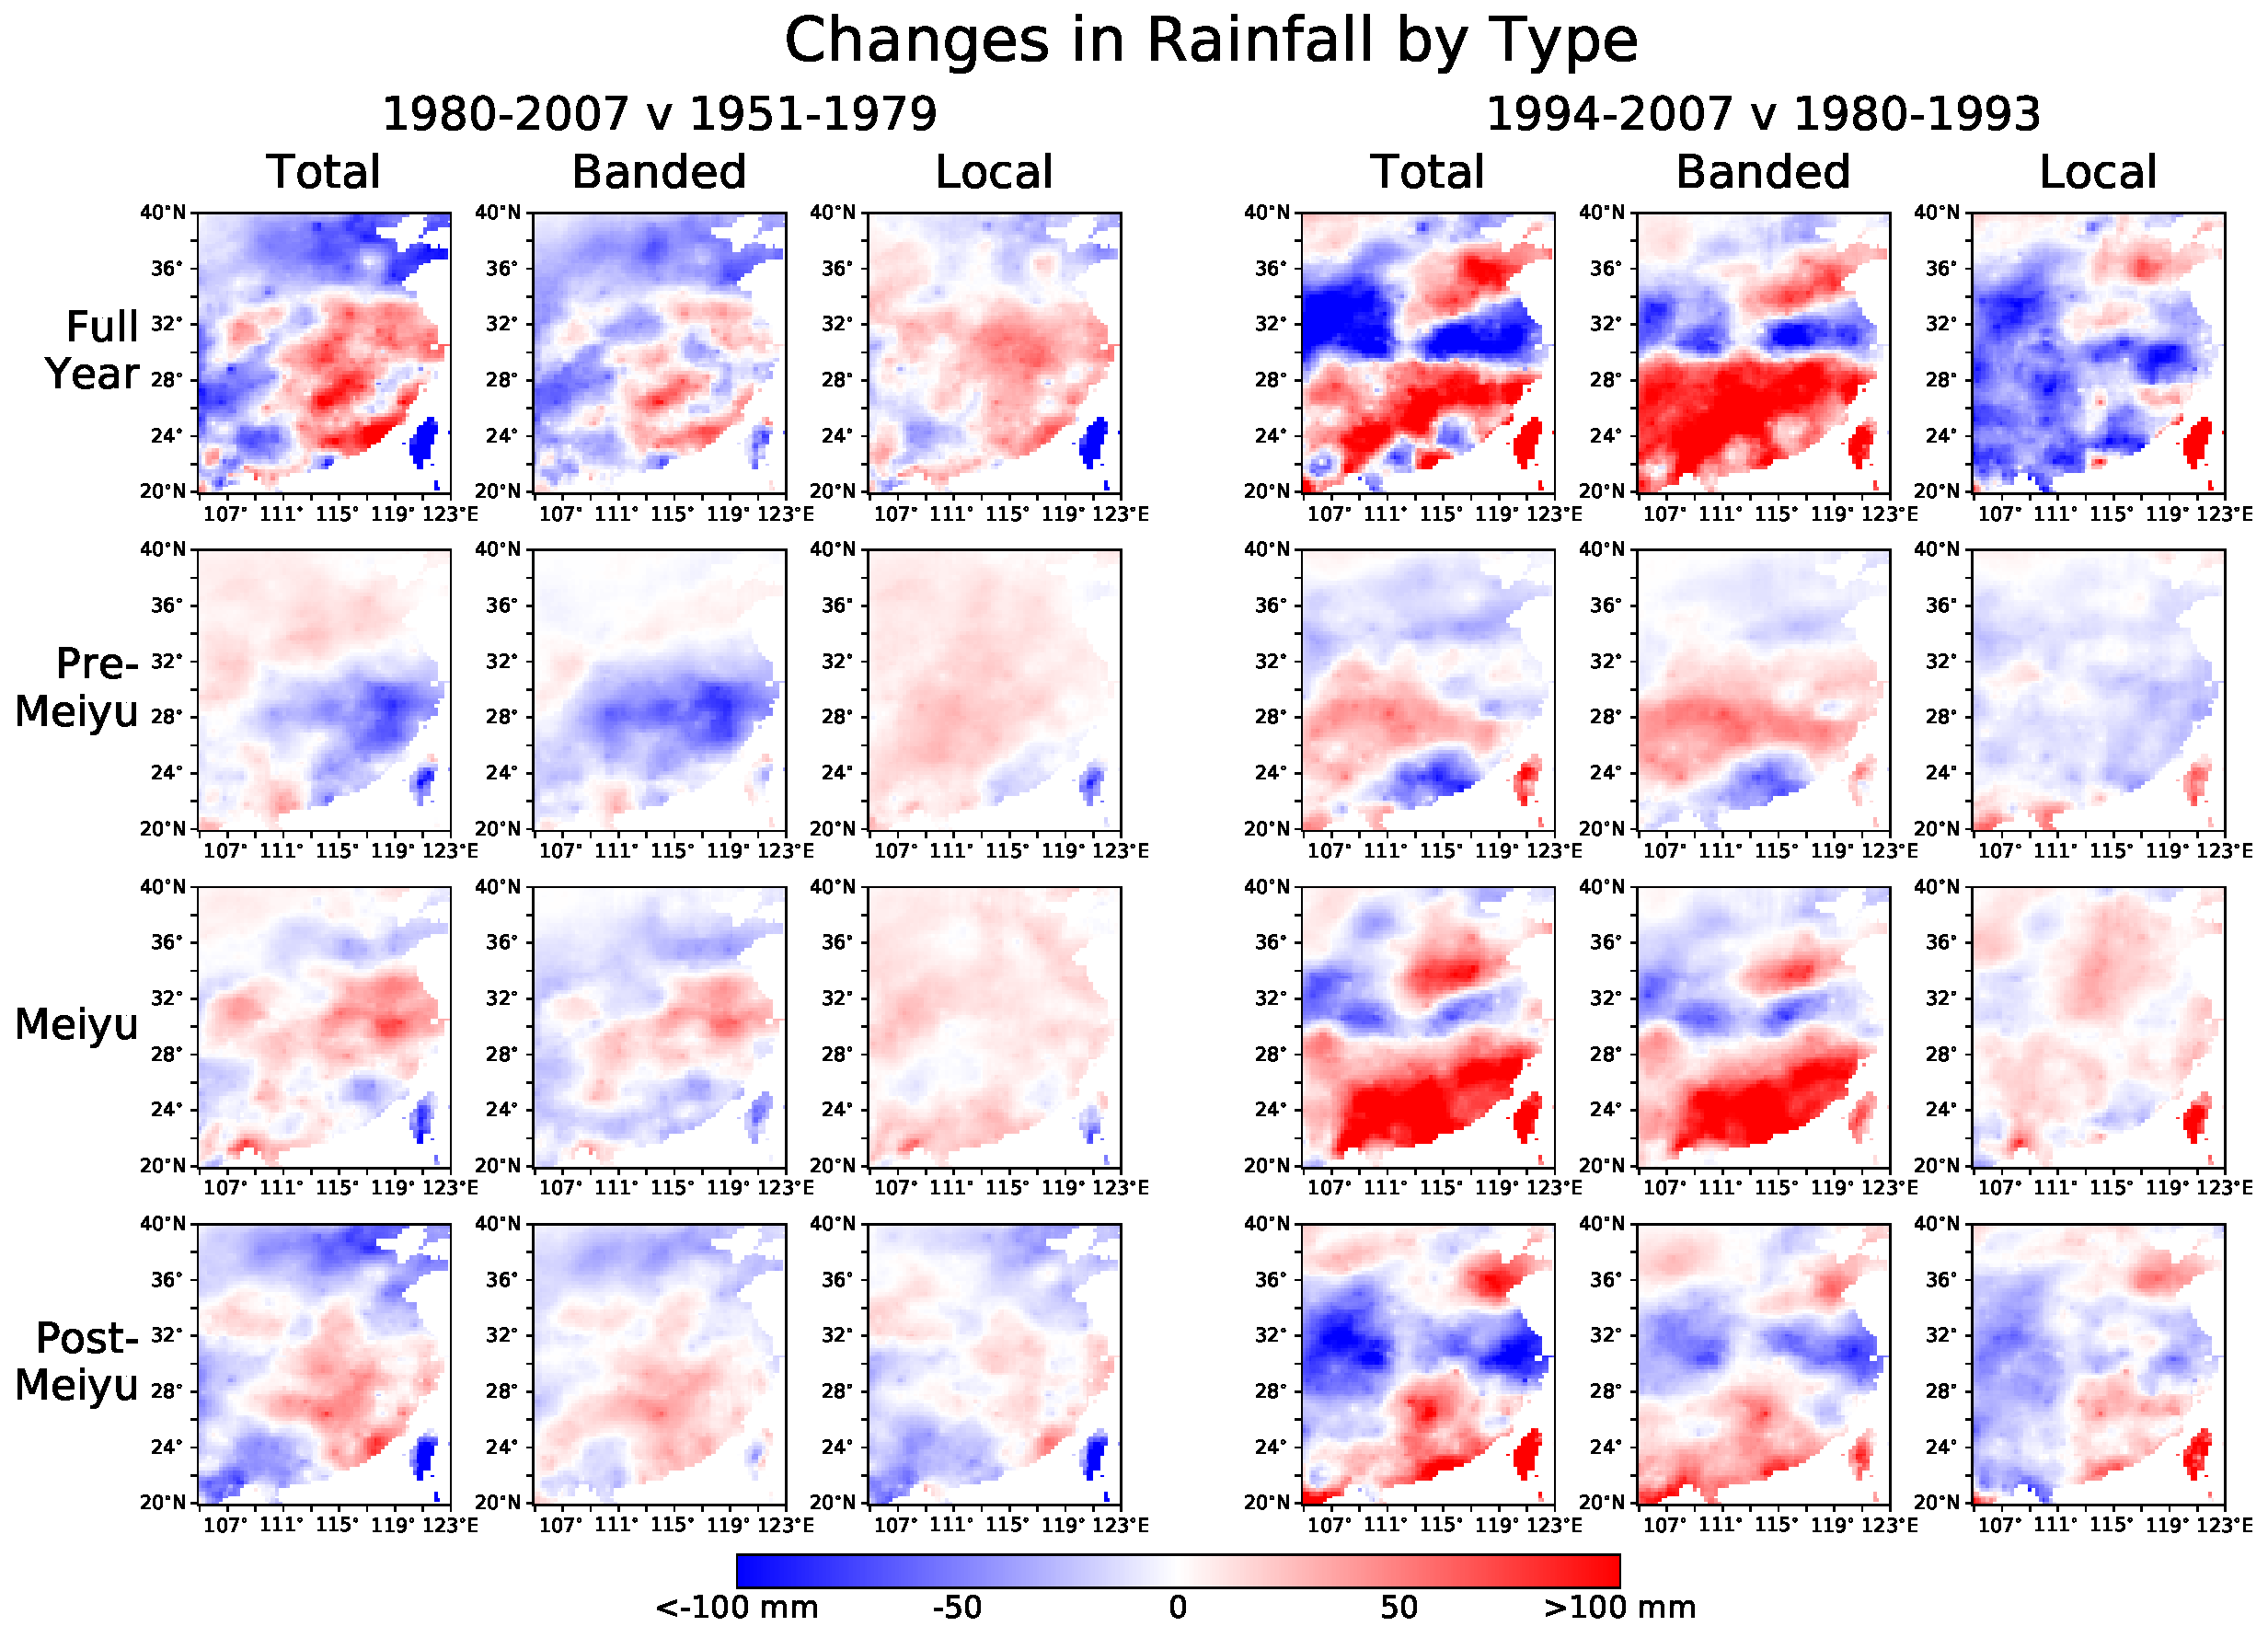
\includegraphics[width=17.8cm]{Figures/changes_by_type}
\caption{Changes in total, banded and local rainfall for full year, Pre-Meiyu (days 121-160), Meiyu (days 161-200) and Post-Meiyu (days 201-273), comparing time periods 1980-2007 to 1951-1979 (left) and 1994-2007 to 1980-1993 (right). \textit{Banded} rainfall consists of all rainfall falling within 4$^{\circ}$ of a rainband axis and rainfall at any other adjacent point exceeding 10 mm day$^{-1}$. \textit{Local} rainfall includes all rainfall not meeting these criteria.}
\label{fig:type_changes}
\end{figure*}

\subsection*{Banded versus Local Rainfall}	
	
	Figure~\ref{fig:type_climo} shows that banded rainfall constitutes at least 40\% of yearly total for all of mainland China east of 105$^\circ$E between 21$^\circ$N and 37$^\circ$N, over 60\% for most of central China, and up to 74\% in the vicinity of Jiangxi Province (28$^\circ$N, 116$^\circ$E). Thus, banded rainfall is an essential component of East China's yearly rainfall budget. Banded rainfall constitutes the majority of rainfall during the Pre-Meiyu and Meiyu, but not the Post-Meiyu. While banded rainfall undergoes a dramatic seasonal northward progression from Pre-Meiyu to Post-Meiyu, the spatial distribution of local rainfall remains largely the same between seasons. Topographic features such as the South China/Qinling mountains and Sichuan Basin anchor regional maxima of local rainfall. Banded rainfall only constitutes a noticeable fraction of Taiwanese rainfall during the Pre-Meiyu. In fact, the term Meiyu season as used in Taiwan refers to late May \citep{Chen1994,Xu2009}, not June 10-July 19  as in our study.

%%FIGURE 4 Significance of attribute changes in rainbands between decades
\begin{figure}[h]
\centering
\noindent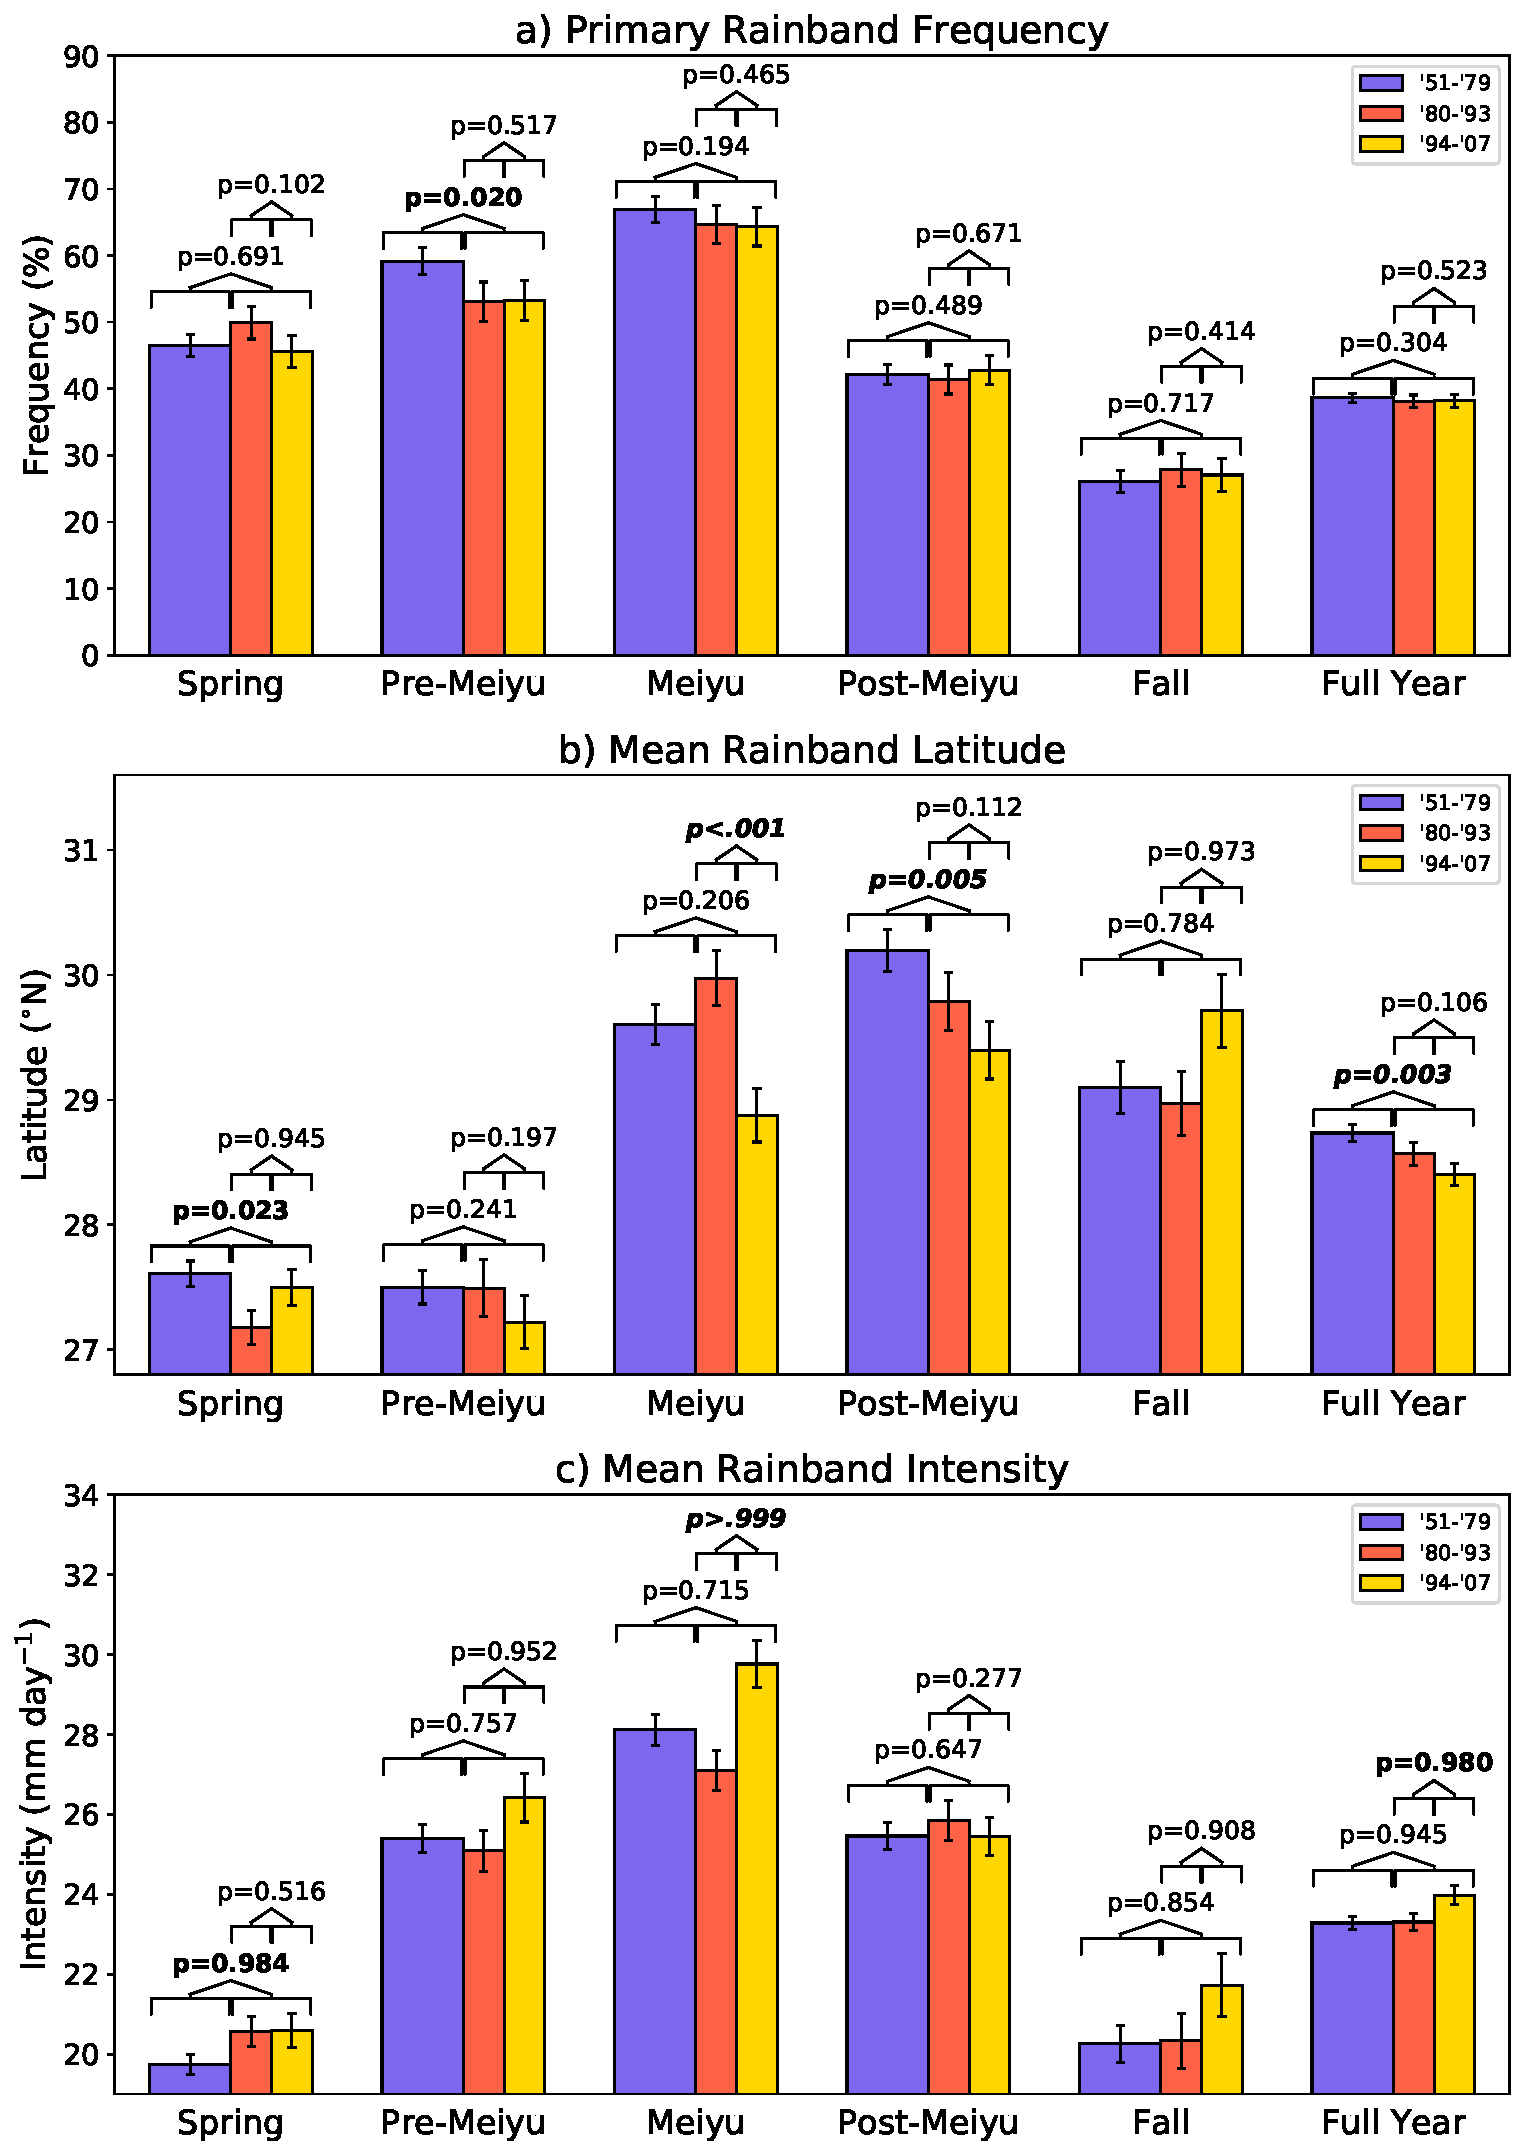
\includegraphics[width=\linewidth]{Figures/bars}
\caption{Significance of decadal changes in a) Rainband frequency, b) Rainband latitude and c) Rainband intensity between decades.}
\label{fig:bars}
\end{figure}	

\section*{Decadal Changes}

	Spatial changes in rainfall between sets of years for key time periods are shown in Figure~\ref{fig:type_changes} and decomposed into banded and local rainfall changes. Figure~\ref{fig:hov_changes} similarly shows zonally averaged banded and local rainfall changes for the entire year in Hovm\"oller plot format, as well as changes in rainband intensity and frequency at each latitude. Finally, Figure~\ref{fig:bars} uses bootstrapping to determine the significance of the overall changes in rainband latitude, frequency and intensity during key time periods. Results for 1980-2007 versus 1951-1979 and 1994-2007 versus 1980-2007 are discussed below; each set of decadal changes has previously been reported in \citep{Gong2002} and \citep{Kwon2007,Wu2010,Yim2013}.
	
\subsection*{1980-2007 versus 1951-1979}

	Examining the changes in yearly rainfall between 1980-2007 and 1951-1979, a meridional dipole is visible between northeastern and southeastern China in Figure~\ref{fig:type_changes}, a phenomenon known as the South Flood-North Drought. Pronounced regional shifts are also visible in Taiwan, South Korea and parts of Japan. Partitioning these changes into a banded and local component, two observations can be made: 1) banded and local rainfall changes appear uncorrelated; 2) changes in total rainfall are predominantly contributed by changes in \textit{banded} rainfall}, except in Taiwan. This again suggests that banded and local rainfall reflect different rainfall mechanisms. Banded rainfall anomalies are concentrated in summer, when rainbands are most frequent.
	
	In northeastern China, yearly rainfall totals after 1980 decreased due to a decline in banded rainfall during the Post-Meiyu (July 20-Sep 30). In southeastern China, a corresponding increase in banded rainfall during the Post-Meiyu is offset by a decline in rainfall during the Pre-Meiyu, such that the yearly change is not statistically significant. Instead, the seasonality of southeastern China rainfall has changed, with later pre-Meiyu onset and more intense Meiyu and Post-Meiyu seasons. 
	
	Changes in banded rainfall can further be attributed to changes in frequency or intensity. In Figure~\ref{fig:hov_changes}, we observed that changes in banded rainfall between 1980-2007 and 1951-1979 are dominated by changes in \textit{frequency}, while no significant changes in intensity are found, contrary to the findings of \cite{Yu2010}. The probability of observing a rainband during the Pre-Meiyu declined from $59.1\% \pm 2.0\%$ to $53.0\% \pm 2.1\%$ ($p=0.020$; Figure~\ref{fig:bars}), leading to a 2 mm day$^{-1}$ daily deficit in banded rainfall.
	
	Changes in banded rainfall during the Post-Meiyu can also be described as a meridional shift in mean latitude. Mean rainband latitude shifted from $33.6^\circ \textrm{N} \pm .3^\circ$ during 1951-1979 southward to $32.9^\circ \textrm{N} \pm .3^\circ$ during 1980-2007 ($p=.0049$; Figure~\ref{fig:bars}). If we repeat the analysis only for rainbands north of 27$^\circ$N (southeastern China is subject to typhoons during the post-Meiyu, which obey different dynamics and may skew statistics), a p-value of $p=.0003$ is obtained. A Kolmogorov-Smirnov (KS) and Anderson-Dearing (AD) tests also both confirm that the change in overall distribution of latitude is statistically significant.
	
	In summary, the South Flood-North Drought meridional dipole results from changes in the frequency of banded rainfall, in particular during the pre-Meiyu and post-Meiyu. The pattern of change in banded rainfall frequency during the post-Meiyu can be described as a statistically significant shift in latitude.
	
	
%%FIGURE 5 Changes in rainfall by type in Hovmoller form
\verb|
\begin{figure*}[tp]
\centering
\noindent
\includegraphics[width=17.8cm]{Figures/hov_summary}
\caption{15-day running mean of the change in a) and b) total rainfall; c) and d) banded rainfall; e) and f) rainband frequency; and g) h) rainband intensity, zonally averaged by latitude over 110-123$^{\circ}$E, comparing years 1980-2007 to 1951-1979 (a,c,e,g) and 1994-2007 to 1980-1993 (b,d,f,h). All changes shown are significant at a 95\% level, and significance exceeding a 99\% level is contoured in gray, as calculated by a moving blocks bootstrap with block length of 2 days and 2,000 iterations. Zonal rainfall averages \textit{exclude} rainfall occurring over Taiwan because the magnitude of changes over the island dwarf changes on the mainland.}
\label{fig:hov_changes}
\end{figure*}
	
\subsection*{1980-1993 versus 1994-2007}
	
	Decadal rainfall changes between these two time periods are again dominated by changes in banded rainfall. We can further pinpoint changes in rainband \textit{intensity} as the primary origin of rainfall changes between 1994-2007 and 1980-1993. Rainbands have intensified year round (from $23.3 \pm .2$ mm day$^{-1}$ to $24.0 \pm .2$ mm day$^{-1}$, $p=.980$), with changes concentrated during Meiyu season ($27.1 \pm .5$ mm day$^{-1}$ to $29.8 \pm .6$ mm day$^{-1}, p=.9997)$). These intensity changes are concentrated in southeastern China (Figure~\ref{fig:hov_changes}d), leading to increased yearly rainfall totals south of 30$^{\circ}$N. The change in the probability distribution of intensity was also found to be significant with $p<.001$ (cf Supplement). We also note that the mean latitude of rainbands during Meiyu season shifted from $30.0^\circ \textrm{N} \pm .2^\circ$ to $28.9^\circ \textrm{N} \pm .2^\circ\ (p=.0003)$. This finding may be independent from the changes in intensity described above, and has likely also contributed to the wettening of southeastern China during 1994-2007.
	
\section*{Conclusion}

	This work has aimed to quantify the role of frontal storms in the yearly rainfall climatology of eastern China. We used the Rainband Detection Algorithm (RDA), a recursive image processing algorithm, to compile a 57-year catalog of daily rainband occurrence over China and the properties of each event, such as latitude, intensity, tilt, width and length. Over 50\% of yearly total precipitation is contributed by banded rainfall in most of eastern China. We identify a sequence of 5 stages of frontal precipitation, each with preferred position, frequency and strength of frontal rainfall: 1) the Spring Rains (March 1-April 30); 2) the Pre-Meiyu (May 1-June 9); 3) the Meiyu (June 10-July 19); 4) the Post-Meiyu (July 20-September 30) and 5) the Fall Rains (October 1-November 16) (Figure~\ref{fig:hov_climo}). The climatological transitions from one period to the next are marked by sharp changes in rainband frequency, latitude and intensity. Simpler alternative metrics of eastern China rainfall fail to reproduce most of these features (Figure S7-S8). Banded rainfall peaks during Meiyu season (late June), while local rainfall peaks during the Post-Meiyu (early August). We argue that these reflect different causal mechanisms (large-scale convergence versus local heating).
	
	Decadal changes in rainfall in eastern China are primarily due to changes in banded rainfall, as opposed to local rainfall (Figures~\ref{fig:type_changes}). A decrease in northern China rainband \textit{frequency} was the principal contributor to drought during 1980-2007 relative to 1951-1979 (Figure~\ref{fig:hov_changes}; $p=<.001$). The start of the rainy season over the Yangtze Valley was also postponed due to a decline in rainband frequency ($p=0.02$). Changes during 1994-2007 versus a 1980-1993 baseline are instead dominated by rainband \textit{intensity} changes during Meiyu season with no change in frequency ($p>.999$). We suggest that the two shifts detailed in this study may result from two different causal mechanisms.
	
	Past authors have attributed these decadal rainfall changes to a combination of anthropogenic forcing\citep{Xu2001,Li2010,Zhao2010} and natural variability\citep{Zhang1999,Xin2006,Lei2014}. In particular, authors have focused on the proliferation of black carbon aerosols in conjunction with Asia's industrialization \citep{Menon2002,Fan2012,Streets2013}. High PM10 aerosol concentration (diameter l $<\mu m$) has been correlated with increased medium-to-heavy rainfall and decreased light rainfall \citep{Choi2008,Wang2016}, possibly linked to the intensity changes shown in this study. Global warming may also affect the East Asian monsoon via other climate components including Pacific and Indian Ocean SST \citep{Gong2002,Qu2012}, the ENSO cycle \citep{Xie2010} and the annual cycle of the East Asian tropical jet \citep{Yu2007,Park2014,Chiang2015}.
	
	It is essential to understand whether the South Flood-North Drought pattern will persist under \nth{21}-century warming. A permanent change would have major humanitarian impacts on densely-populated eastern China, where a sizable fraction of the population depends on agriculture for subsistence. The CMIP5 (Climate Model Intercomparison Project) model suite contained in the Intergovernmental Panel on Climate Change's Fifth Assessment Report (IPCC AR5) does not agree on the sign of future summer rainfall changes in East Asia \citep{Christensen2011}. Depending on the relative roles of global warming, aerosols and natural variability in the East China rainfall changes studied in this paper, anomalies may be exacerbated or return to their \nth{20} century baseline. Since anthropogenic aerosol concentration is projected to decline during the \nth{21} century \citep{Westervelt2015}, the effects of continued global warming will predominate, potentially with a distinct "thumbprint" of rainfall intensity and frequency changes \citep{Trenberth2003,Trenberth2011a,Pendergrass2014b,Wang2016}. Improved attribution of \nth{20}-century East China rainfall changes may therefore improve future projections.

\matmethods{

\subsection*{APHRODITE Rainfall}

	The APHRO\_MA\_V1101 product from APHRODITE (Asian Precipitation - Highly-Resolved Observational Data Integration Towards Evaluation of the Water Resources) includes 57 years (1951-2007) of continental daily rainfall (PRECIP product) on a .25$^{\circ} \times .25^{\circ}$ grid over 60$^{\circ}$-150$^{\circ}$E and 15$^{\circ}$S-55$^{\circ}$N \citep{Yatagai2012}, as well as a daily map of reporting weather stations on the same grid (RSTN product), for each day from 1 January 1951 to 31 December 2007 (20,819 days total). Values are reported over land only. We focus on the subregion 105$^{\circ}$E-123$^{\circ}$E and 20$^{\circ}$N-40$^{\circ}$N (``East China'') where rainbands are known to occur frequently, especially during Meiyu season (early June to late July). The network of stations remains dense (100-200 km spacing) through time, such that rainbands are clearly resolved and we are not concerned about potential artifacts from changes in station density. APHRODITE's resolution cannot capture some features visible in TRMM satellite data \citep{Xu2009}, but we employ it here in order to study decadal change. We use the words ``rainfall'' and ``precipitation'' interchangeably in the rest of this work since most precipitation in the study region consists of rain, although snow is common in northeastern China during winter.
	
\subsection*{Rainband Detection Algorithm (RDA)}

	Rainbands are observed year-round in East China (hereafter defined as the subregion inside of 105-123$^{\circ}$E and 20-40$^{\circ}$N). RDA defines a rainband as a continuous chain of longitudinal rainfall maxima in excess of 10 mm day$^{-1}$ spanning at least 5$^{\circ}$ of longitude. On each day where a rainband is present, RDA attempts to model it as a straight line by performing a weighted linear fit of the latitude of maximum rainfall at each longitude, using intensity as weighting and discarding outliers far from the centroid of precipitation, and then recursively repeats the fit using an increasingly narrow window around the previous best guess (Figure S4). The exact algorithm is described in greater detail in \citep{Day2016}.  
	
	Once a fit is achieved, the following key metrics are calculated:
				
 \begin{itemize}
	 
	\item \textit{Quality Score (Q)}: The fraction of daily total East China rainfall that falls within $2.5^{\circ}$ degrees of the best estimate line (Figure S3).
	 
	 \item \textit{Latitude}: The latitude of the best fit line at 115$^{\circ}$E. 
	 
	 \item \textit{Intensity}: Mean rainfall of all ``rainband points'' (any point along the best fit line where daily rainfall exceeds 5 mm day$^{-1}$).
	 
	 \item \textit{Length}: Total number of rainband points (units of degrees longitude)
	 
	 \item \textit{Width}: Mean distance between half-maxima ($int_{max}$/2) on either side of each rainband point (units of degrees latitude).
	 
\end{itemize}
	
	 In some cases two rainbands exist simultaneously. The more intense of the two is termed ``primary,'' and the weaker ``secondary.'' Secondary rainbands are detected by first removing all ``banded rainfall'' associated with the primary rainband (defined as all rainfall falling within 4$^{\circ}$ of a rainband axis, and any other adjacent points where rainfall exceeds 10 mm day$^{-1}$; Figure S1). If two rainbands coexist, conditional quality scores $Q_1$ and $Q_2$ are calculated. $Q_1$ is defined as the fraction of daily East China rainfall that fell within $2.5^{\circ}$ degrees of the primary rainband \textit{after removing secondary rainband rainfall}, and vice-versa for $Q_2$.

\subsection*{Quality Control}

	 Out of 20,819 days, at least one rainband was detected on 11,228 days, and two rainbands on 1,116 days. Subsequently, we use quality scores $Q$, $Q_1$ and $Q_2$ to identify poor fits. We also use the ``Taiwan fraction'' $TW$ (percentage of daily East China rainfall falling over the island of Taiwan, 120-$122^{\circ}$E and 22-$26^{\circ}$N) to identify days when Taiwan receives far more rain than East China, skewing the RDA best fit (Figure S1). Fits on days where $TW > 20\%$ are thrown out. Subsequently, one of two criteria must be met:
	
	\begin{enumerate} 
	
	\item If $Q>.6$, the fit is deemed successful (7,522 days, 67.0\% of total fits; Figure S2). If $Q_2$ is also greater than .6, the day will be classified as a double rainband day (Type I double rainband; 232 cases). 3.1\% of days where $Q>.6$ also achieve $Q_2>.6$.
		
	\item If $Q<.6$, the fit is discarded unless two rainbands are detected and conditional quality scores $Q_1$ and $Q_2$  both exceed .6. In such cases, the presence of multiple rainbands of comparable intensity initially obscures the goodness of fit (Figure S4). Such days are also classified as double rainband days (Type II double rainband; 466 cases).
	
	\end{enumerate}
		
	The use of conditional quality scores $Q_1$ and $Q_2$ adds 466 double rainband fits (6.2\% of all successful fits) that would otherwise have been missed due to $Q<.6$. 33.2\% of double rainband days are Type I ($Q>.6$) and 66.8\% Type II ($Q<.6$) as defined above. Double rainbands are more common during certain months, particularly July-September.

\subsection*{Banded and Local Rainfall}
	
	We further classify all rainfall on each day as either \textit{banded} (falls within a rainband) or \textit{local}. \textit{Banded} rainfall consists of all rainfall falling within 4$^{\circ}$ of latitude of a rainband axis and any other adjacent points where rainfall exceeds 10 mm day$^{-1}$ (Figure S4). This partition is based on our knowledge of the physical mechanisms of rainfall in eastern China: Banded rainfall results from large-scale convergence due to frontal conditions and the propagation of westerly storms across thousands of miles \citep{Molnar2010,Day2016}, whereas local rainfall most likely results from mechanisms with shorter length scales, such as convective self-buoyancy and orographic rainfall. We cannot rule out that multiple mechanisms are capable of producing banded rainfall, or that the mechanism of formation varies by season.

} % end of materials and methods

\showmatmethods % Display the Materials and Methods section

\acknow{	APHRODITE precipitation data is publicly available at \url{http://www.chikyu.ac.jp/precip/index.html}. The rainband detection algorithm was written in MATLAB and subsequent data analysis carried out within Jupyter Notebook. The author's data analysis is freely available on Github. Ferret, a NOAA product, was used for some figure generation and is freely available at \url{http://ferret.pmel.noaa.gov/Ferret/}. A full database of rainband statistics from 1 January 1951 to 31 December 2007 and associated MATLAB and Ferret codes used to produce results are available on the author's Github repository. This work was supported by NSF grants EAR-0909195 and EAR-1211925, which allowed the presentation of preliminary results in conference settings, as well as DOE grant DE-SC0014078. We also acknowledge NSFC (National Natural Science Foundation of China) grant \#40921120406 for enabling collaboration with Professor Yanjun Cai of IEECAS in Xi'an, which led to the present work. We thank Jinqiang Chen and an anonymous reviewer for valuable suggestions on a previous version of this manuscript.}

\showacknow % Display the acknowledgments section

% \pnasbreak splits and balances the columns before the references.
% If you see unexpected formatting errors, try commenting out this line
% as it can run into problems with floats and footnotes on the final page.
\pnasbreak

% Bibliography
\bibliography{RDA_biblio_final}

\end{document}